\section{Results \& Discussion}

This section presents the detailed findings and results of our experiments of using various unsupervised anomaly detection models for the task of identifying faulty solder joints in \gls{pcb}. The models which we have evaluated here are PatchCore(section \ref{subsec:patchcore}), \gls{dfm}(section \ref{subsec:dfm}), \gls{dfkde}(section \ref{subsec:dfkde}), EfficientAD(section \ref{subsec:efficientad}), FastFlow(section \ref{subsec:fastflow}), which uses different hyper parameters, feature extraction backbones and its layers. Our aim is the study the effectiveness of these models in comparison to the current baseline models used by Siemens \gls{yolo}(section \ref{subsec:yolo}), while also the factors affecting their performances.

\subsection{Overall Performance of Models}

The table \ref{tab:overall model accuracy} and the bar chart \ref{fig:bar chart models accruacy} represents the overall accuracy performance of each model, which gives an initial overview of how these models compare in terms of how they classify anomalies correctly.

\begin{table}[ht!]
    \centering
    \begin{tabular}{|l|l|}
        \hline
        \textbf{Model} & \textbf{Accuracy} \\ \hline
        \textbf{Yolov8-L} & \textbf{95\%} \\ \hline
        \textbf{Yolov8-M} & \textbf{93.75\%} \\ \hline
        \textbf{PatchCore} & \textbf{91.25\%} \\ \hline
        Deep Feature Modeling(DFM) & 72.85\% \\ \hline
        Deep Feature Kernel Density Estimation(DFKDE) & 70.71\% \\ \hline
        FastFlow & 66.87\% \\ \hline
        EfficientAD & 60\% \\ \hline
    \end{tabular}
    \caption{Overall comparison of different models accuracy}
    \label{tab:overall model accuracy}
\end{table}

The chart \ref{fig:bar chart models accruacy} provides a graphical representation of the same data of each models accuracy, where we can clearly visualize the performance of different models. As can be seen in table \ref{tab:overall model accuracy} and bar chart \ref{fig:bar chart models accruacy} that the baseline model \gls{yolo}v8-L achieves the highest accuracy of 95\%, while the best performing unsupervised model is PatchCore closely following with an accuracy of 91.25\%, with only a 2.5\% difference in the accuracy of different size of baseline model \gls{yolo}v8-M. Other models such as \gls{dfm}, \gls{dfkde}, FastFlow, and EfficientAD shows moderate performance. Here none of the unsupervised anomaly detection models could over take the supervised baseline model, one of the reasons for this is that the baseline model was trained in supervised fashion, where it had access to all the labels of the image dataset. Whereas the anomaly detection models were not given any labels of the images and while training only anomaly free data was used, and it had to figure out on its own which images are anomalous and which images are normal.

\begin{figure}[ht!]
    \centering
    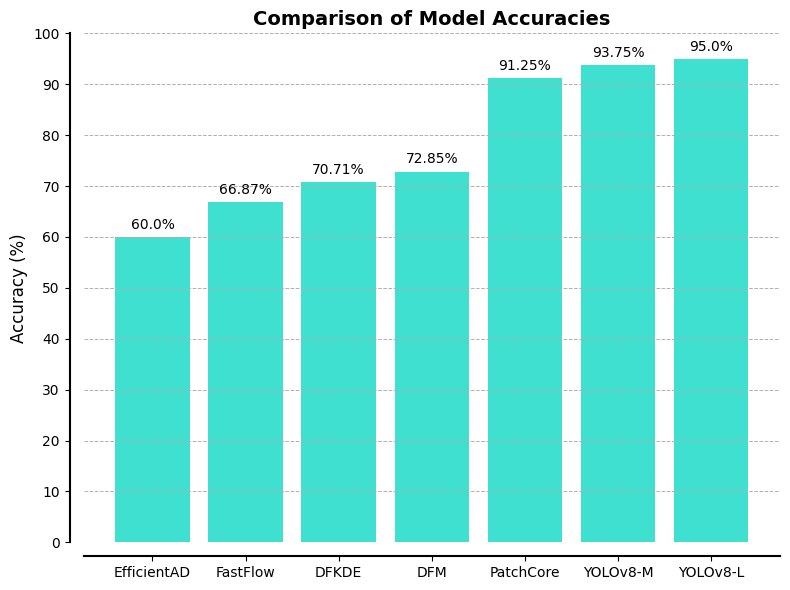
\includegraphics[width=1.1\linewidth]{Rohit_Master_Thesis//Images/bar_chart_model_acc.png}
    \caption{Bar chart representation of the different models accuracy like \gls{yolo}(baseline), our approach including PatchCore, \gls{dfm}, \gls{dfkde}, FastFlow, and EfficientAD.}
    \label{fig:bar chart models accruacy}
\end{figure}

\subsection{Model-wise breakdown of results}

\paragraph*{PatchCore : }

\begin{figure}[H]
    \centering
    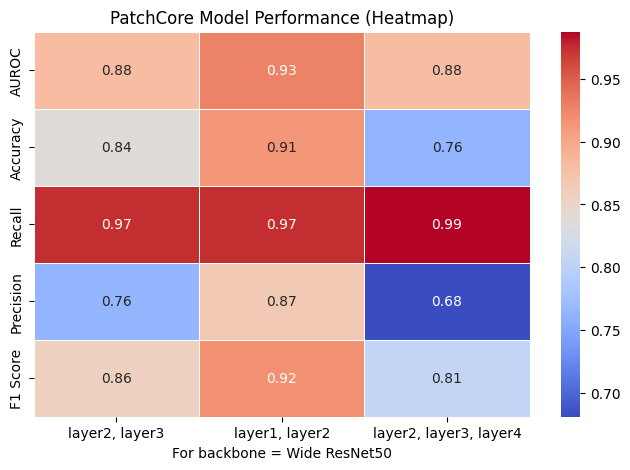
\includegraphics[width=1\linewidth]{Rohit_Master_Thesis//Images/patchcore heatmap.png}
    \caption{PatchCore heatmap for the experiment where backbone "Wide Resnet50" and layers "2, 3" were used.}
    \label{fig:patchcore heatmap}
\end{figure}

\iffalse
\begin{figure}[ht!]
    \centering  
    % First image
    \begin{minipage}{0.6\textwidth}
        \centering
        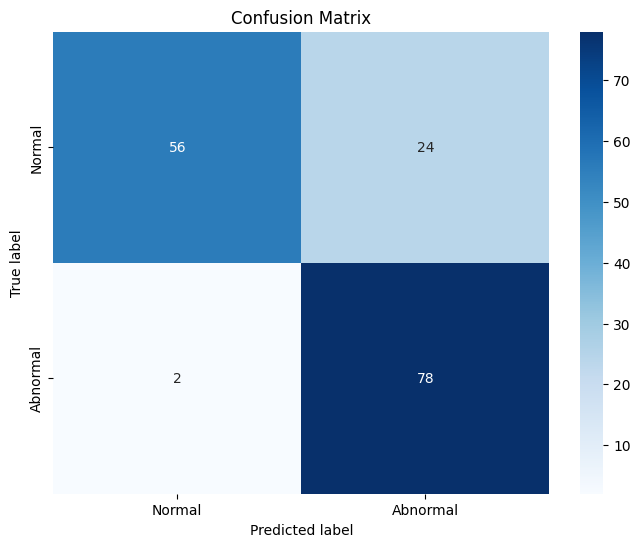
\includegraphics[width=\textwidth]{Rohit_Master_Thesis//Images/patchcore_config1_confusion_matrix.jpg} % Add your image file name here
        \caption{Configuration 1}
    \end{minipage}
    
    \vspace{0.5cm} % Adds vertical space between images
    
    % Second image
    \begin{minipage}{0.6\textwidth}
        \centering
        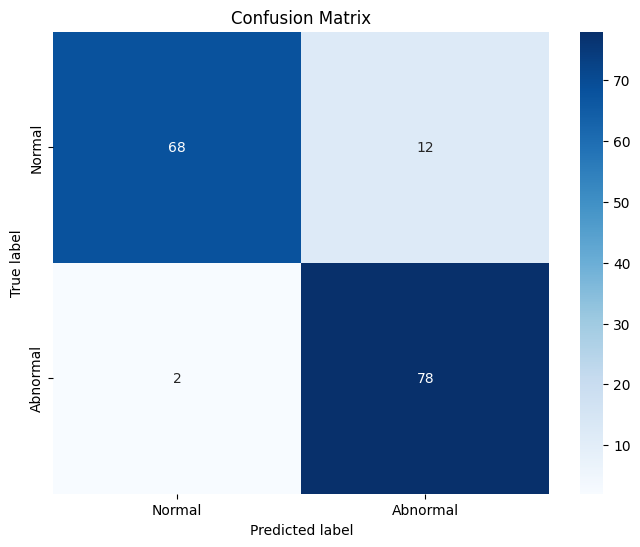
\includegraphics[width=\textwidth]{Rohit_Master_Thesis//Images/patchcore_config2_confusion_matrix.jpg} % Add your image file name here
        \caption{Configuration 2}
    \end{minipage}
    
    \vspace{0.5cm} % Adds vertical space between images
    
    % Third image
    \begin{minipage}{0.6\textwidth}
        \centering
        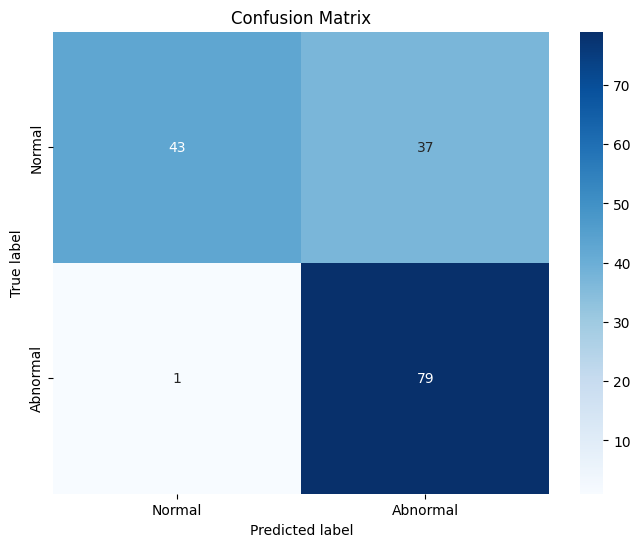
\includegraphics[width=\textwidth]{Rohit_Master_Thesis//Images/patchcore_config3_confusion_matrix.jpg} % Add your image file name here
        \caption{Configuration 3}
    \end{minipage}
    
    \caption{Comparison of Confusion Matrices for Different Configurations.}
    \label{fig:dataset-NG}
\end{figure}
\fi

For this experiment, we employed PatchCore with \texttt{wide\_resnet50\_2} backbone as feature extraction for performing anomaly detection. Firstly the model extracts feature representations from specific layers of the backbone and then compares the patch-level features of test images with those stored in a memory bank built from normal data. PatchCore uses \gls{k-nn} retrival for detecting deviations from nominal behavior by calculating the anomaly score based on the distance between patches from the test image and their closest counterparts in the memory bank. This allows PatchCore to perform well when the labeled data is not abundantly available, this model is explained in much more detail in \ref{subsec:patchcore}.

For the first configuration, we have used backbone \texttt{wide\_resnet50\_2} with layer2 and layer3 as shown in the heatmap \ref{fig:patchcore heatmap}. This configuration achieves an \gls{auroc} score of 0.8816 and an overall accuracy of 83.75\%. The F1-score was relatively strong at 0.8571, suggesting that the model maintained balance between precision and recall. The model had a precision of 0.7647 suggesting that sometimes the model classified normal data as anomalous, which resulted in moderate occurrence of false positive as can be confirmed by the confusion matrix \ref{fig:patchcore config1 confusion matrix}. Whereas, the high recall value of 0.975 indicates that the model was highly accurate in detecting almost all the anomalies as anomalies, with some false negatives as can be seen in the \ref{fig:patchcore config1 confusion matrix}.

\begin{figure}[ht!]
    \centering
    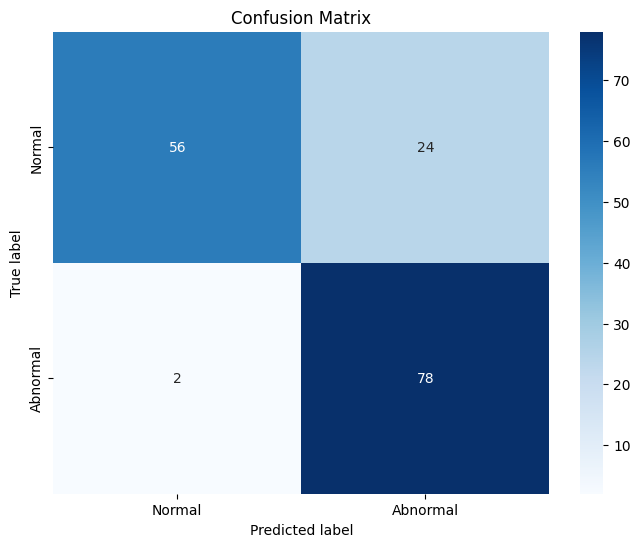
\includegraphics[width=1\linewidth]{Rohit_Master_Thesis//Images/patchcore_config1_confusion_matrix.jpg}
    \caption{Confusion matrix for the first configuration where backbone "Wide Resnet50" and layers "2, 3" were used.}
    \label{fig:patchcore config1 confusion matrix}
\end{figure}

The second configuration resulted in the best overall performance across all metrics, where the feature extraction was carried out by layer1 and layer2 of the same backbone \texttt{wide\_resnet50\_2}. This configuration resulted in a high \gls{auroc} score of 0.9271, with a significant increase in accuracy of 91.25\% as shown in the heatmap \ref{fig:patchcore heatmap}. We also saw improvement in F1-score by about 6.6\% from the previous configuration, reaching 0.9176 indicating an even better balance between precision and recall. The precision improved to 0.8667, indicating a reduction in false positives as can be seen in the confusion matrix \ref{fig:patchcore config2 confusion matrix} where the false positives reduced by 50\% from the first configuration. While the recall remained high but same as the first configuration at 0.975, meaning the model continued to detect almost all anomalies like show in the figure \ref{fig:patchcore config2 confusion matrix}. The improved performance of this configuration can be due to the use of features from the combination of layer1 and layer2, which incorporates the combination of both low-level and mid-level features. As low-level features might allow the model to detect fine-grained details, while layer2 might provide the more complex structures needed to detect anomalies. These features can provide a more richer, and detailed representation of normal data, making the detection of anomalies without overfitting on normal data easier.

\begin{figure}[ht!]
    \centering
    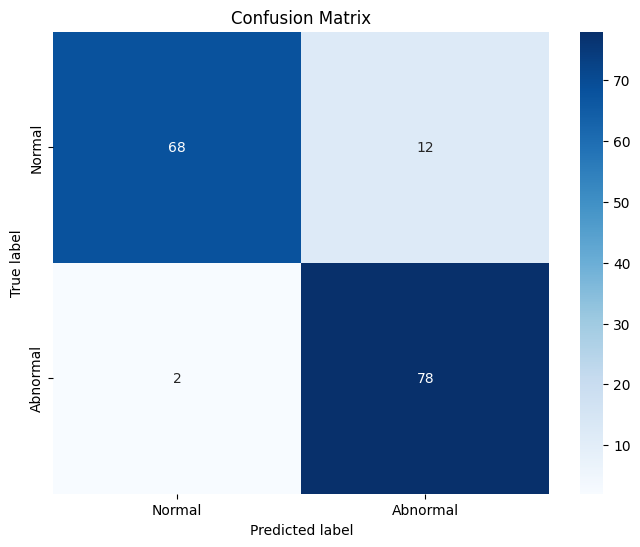
\includegraphics[width=1\linewidth]{Rohit_Master_Thesis//Images/patchcore_config2_confusion_matrix.jpg}
    \caption{Confusion matrix for the second configuration where backbone "Wide Resnet50" and layers "1, 2" were used.}
    \label{fig:patchcore config2 confusion matrix}
\end{figure}

In the third configuration, layer2, layer3, layer4 was used of the backbone \texttt{wide\_resnet50\_2}, it resulted in lower \gls{auroc}score of 0.8807 which is almost equal to the \gls{auroc} score for first configuration, and the accuracy we got is 76.25\% which is the lowest of all the configuration. The F1-score also decreased slightly to 0.8061, due to drop in precision value to 0.6810. This lower precision indicates that the model produced higher number of false positives i.e. more normal images were classified as anomalous as can be seen in confusion matrix \ref{fig:patchcore config3 confusion matrix} where out 0f 80 normal images 37 were classified as anomalous. But the recall was the highest at 0.9875, which means that the model was still able to detect almost all of the anomalies as can been seen in the figure \ref{fig:patchcore config3 confusion matrix} out of 80, 79 were correctly classified as anomalous with only one being misclassified as normal. The inclusion of deeper layers, like layer4 probably introduced more abstract features which may have been less effective for the detection of fine-grained anomalies, resulting in the reduction of overall performance. This configuration highlights the importance of extraction of features from appropriate layers for ensuring balance between detecting true anomalies and avoiding excessive false positives.

\begin{figure}[ht!]
    \centering
    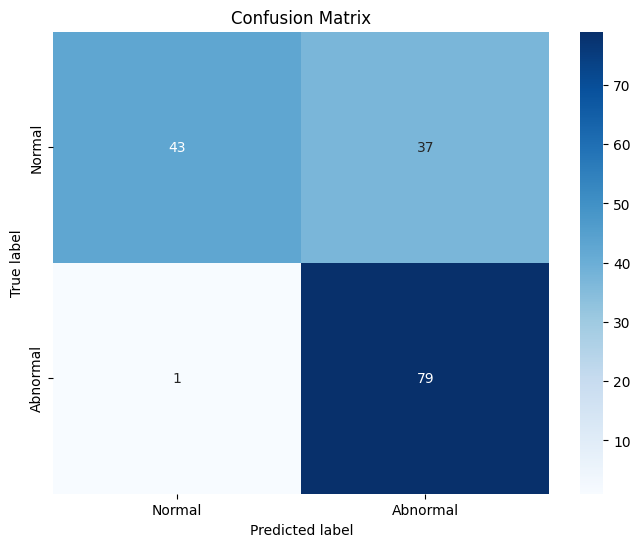
\includegraphics[width=1\linewidth]{Rohit_Master_Thesis//Images/patchcore_config3_confusion_matrix.jpg}
    \caption{Confusion matrix for the third configuration where backbone "Wide Resnet50" and layers "2, 3, 4" were used.}
    \label{fig:patchcore config3 confusion matrix}
\end{figure}

\paragraph*{\gls{yolo} : }Two different model sizes of \gls{yolo}v8 \cite{Ultralytics2024} were evaluated for this experiment: \gls{yolo}v8-M(medium) and \gls{yolo}v8-L(large). Both the models were trained for 200 epochs on the training dataset.

The \textbf{\gls{yolo}v8-L} model which is larger in size and more complex, reached accuracy of 95\% after 200 epochs. The model's high accuracy could be due to its increase in the depth and number of parameters, which allows it to capture more detailed and complex patterns in the dataset. Also it being a supervised model, having access to all the labels while training helps it to learn better and fit the model well to the data.

\begin{figure}
    \centering
    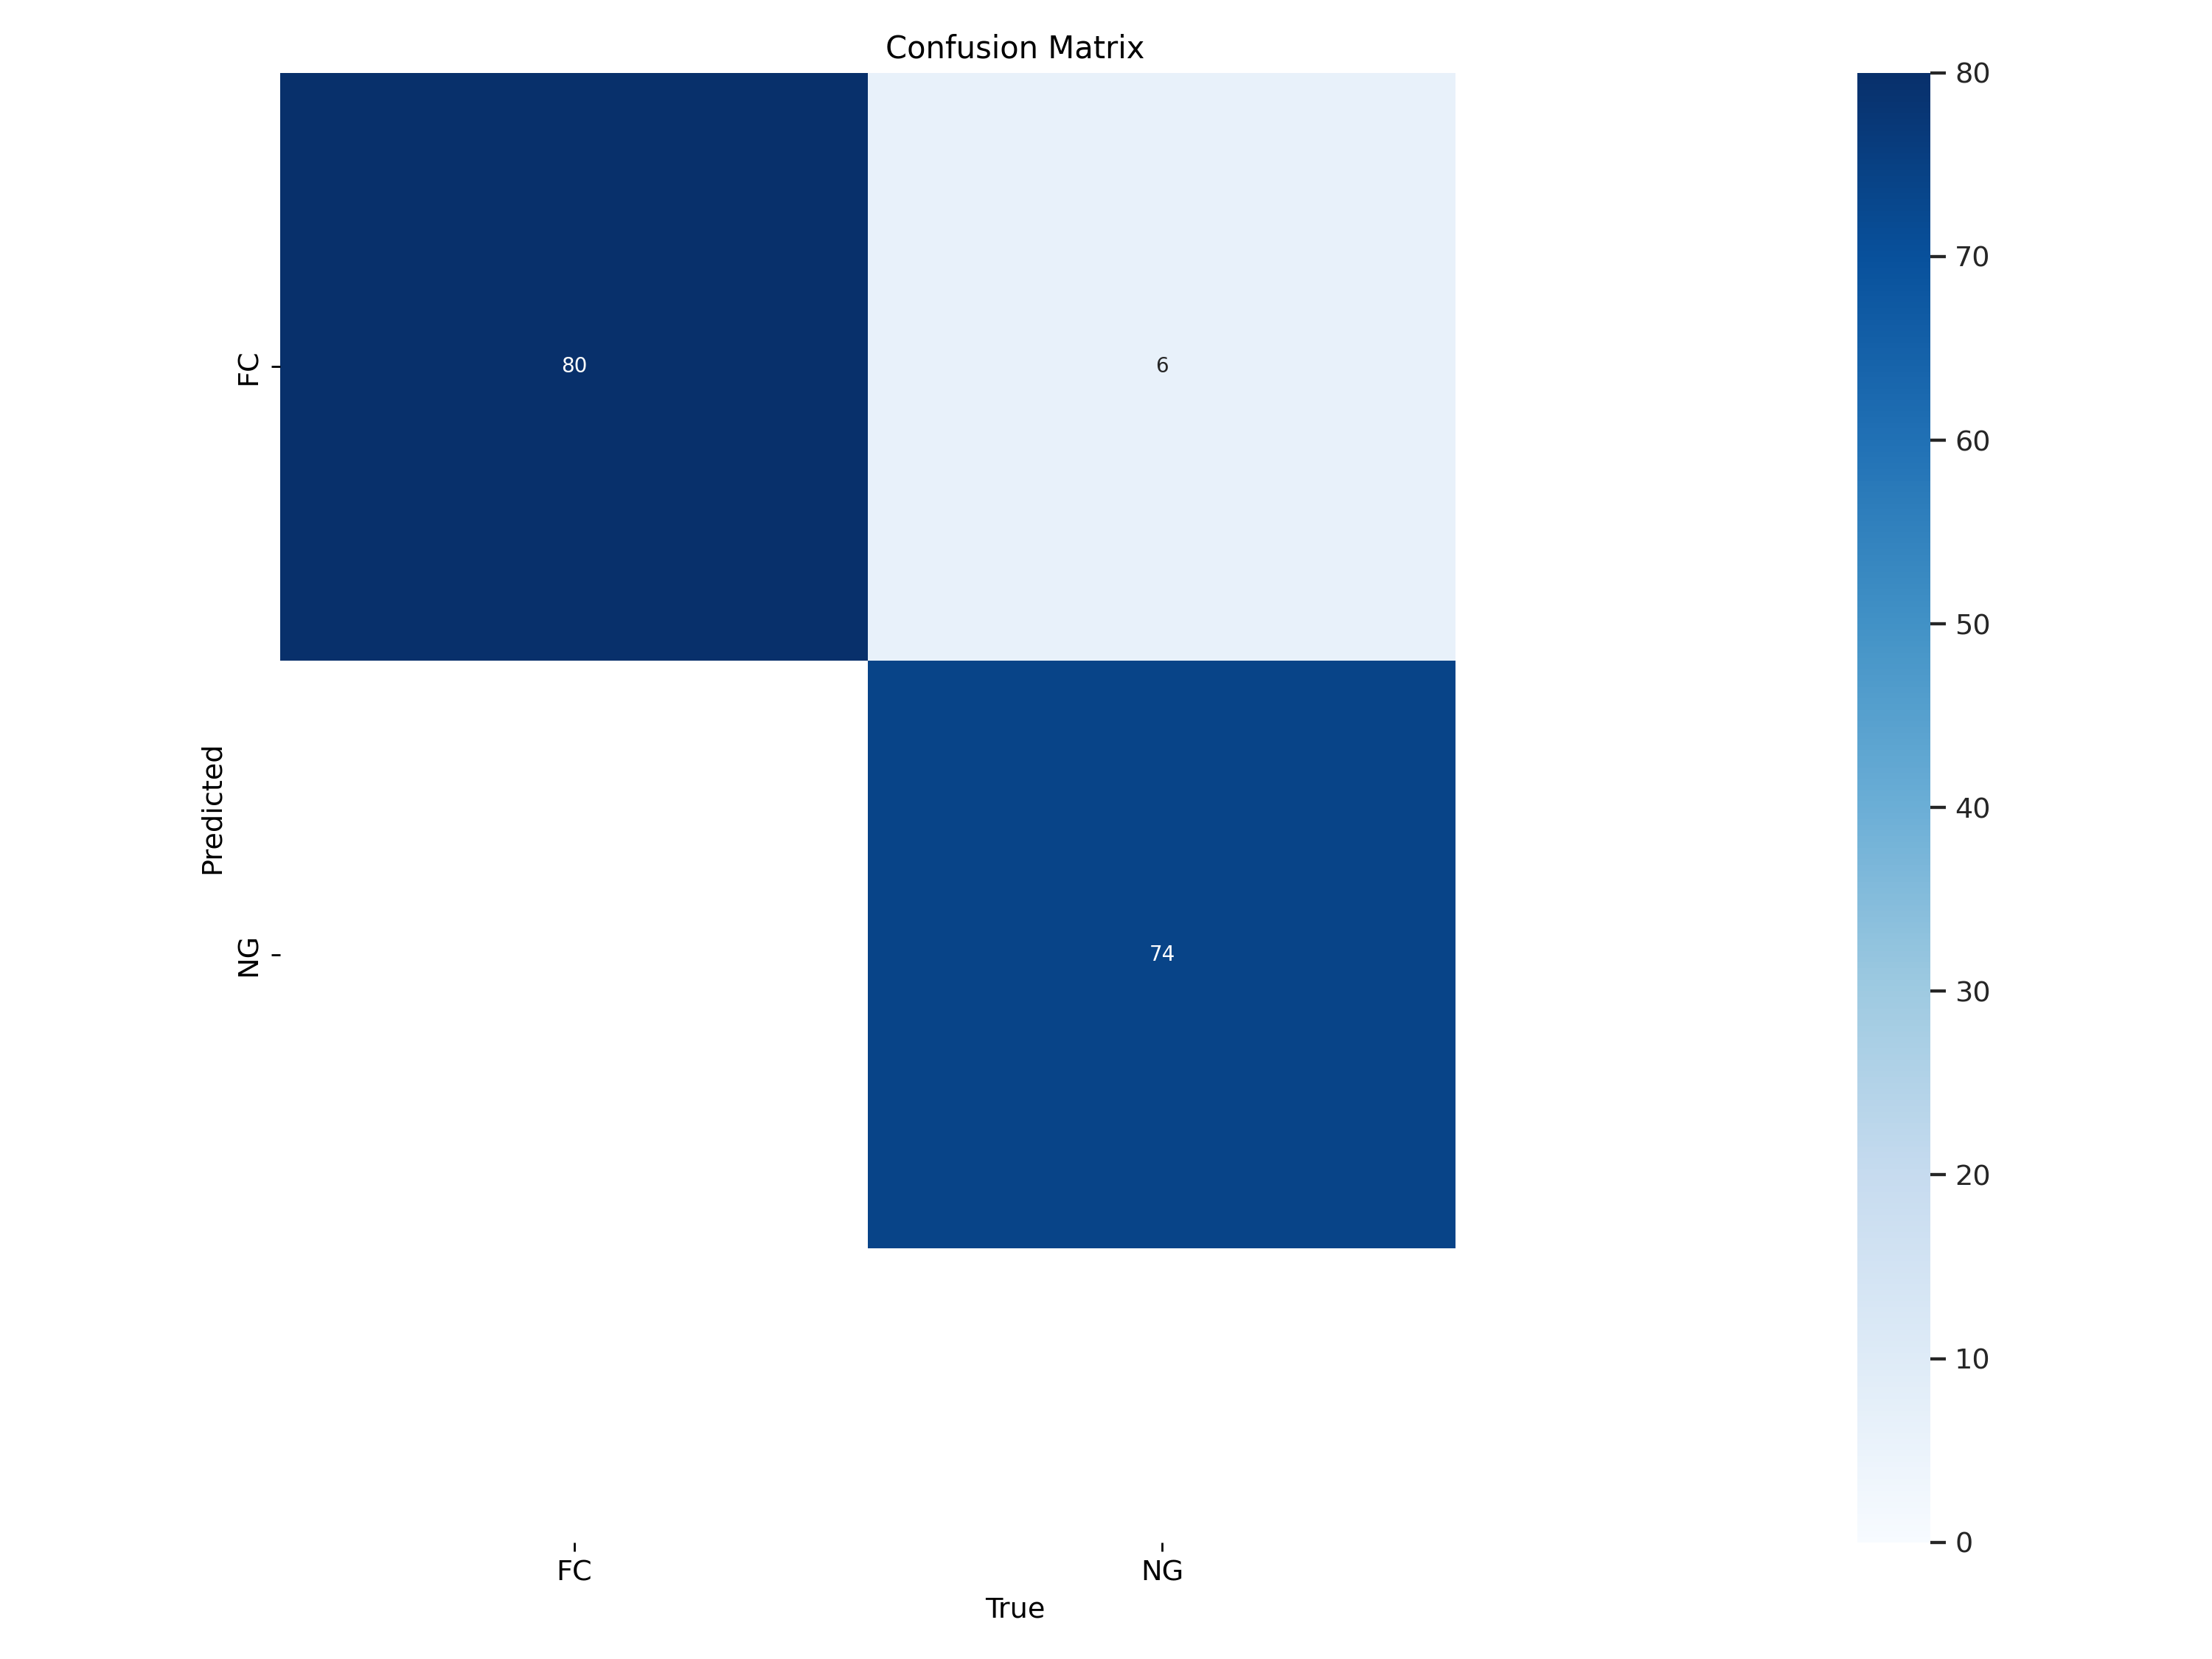
\includegraphics[width=1.3\linewidth]{Rohit_Master_Thesis//Images/yolov8l_confusion_matrix.png}
    \caption{Confusion matrix for the baseline model \gls{yolo}v8-L, its accuracy is 95\%}
    \label{fig:yolov8l confusion matrix}
\end{figure}

The confusion matrix as shown in figure \ref{fig:yolov8l confusion matrix} provides a more detailed look into how well the model performs in classification task. We can see that the model correctly classified all the normal(FC) images as normal, while only 6 were false positive i.e. anomalous(NG) images were classified as normal images, rest of the 74 were correctly classified as NG i.e. True Negatives. These values are consistent with the precision, recall and F1-score results as shown in table \ref{tab:yolov8_performance}. The precision of 1.0 highlights the models reliability in predicting normal(FC) instances, as it didn't make any incorrect predictions for that class. The recall of 0.925, while still quite good, indicates that the model, it misclassified a small number of anomalous(NG) as normal(FC). With the impressive F1-score of 0.9615, shows the models well-rounded performance.

\begin{table}[ht!]
    \centering
    \begin{tabular}{|c|c|c|c|c|}
        \hline
        \textbf{Model} & \textbf{Accuracy} & \textbf{Precision} & \textbf{Recall} & \textbf{F1-score} \\ \hline
        \textbf{YOLOv8-M} & 93.75\% & 0.9867 & 0.925 & 0.9547 \\ \hline
        \textbf{YOLOv8-L} & 95\% & 1.0 & 0.925 & 0.9615 \\ \hline
    \end{tabular}
    \caption{Comparison of YOLOv8-M and YOLOv8-L Model Performance}
    \label{tab:yolov8_performance}
\end{table}

%Probably for discussion section(remember to paraphrase)
%Explanation of Results
%The performance of YOLOv8-L is in line with its design as a larger, more powerful model. The depth and complexity of the YOLOv8-L architecture allow it to capture a wide variety of patterns and features in the data, leading to its high precision and recall. The non-maximum suppression (NMS) technique used in YOLOv8 helps further refine the predictions by ensuring that overlapping bounding boxes are filtered, resulting in more accurate object classification. Additionally, YOLOv8-L's anchor-free detection mechanism improves its ability to generalize across objects of various sizes, contributing to its robustness in detecting NG and FC items.

The \textbf{\gls{yolo}v8-M} model, which is smaller and more lightweight when compared to \gls{yolo}v8-L, reaching an accuracy of 93.75\%. Which is slightly lower than its bigger model as can be seen from the table \ref{tab:yolov8_performance}, but it overall performance was still quite impressive.

\begin{figure}[ht!]
    \centering
    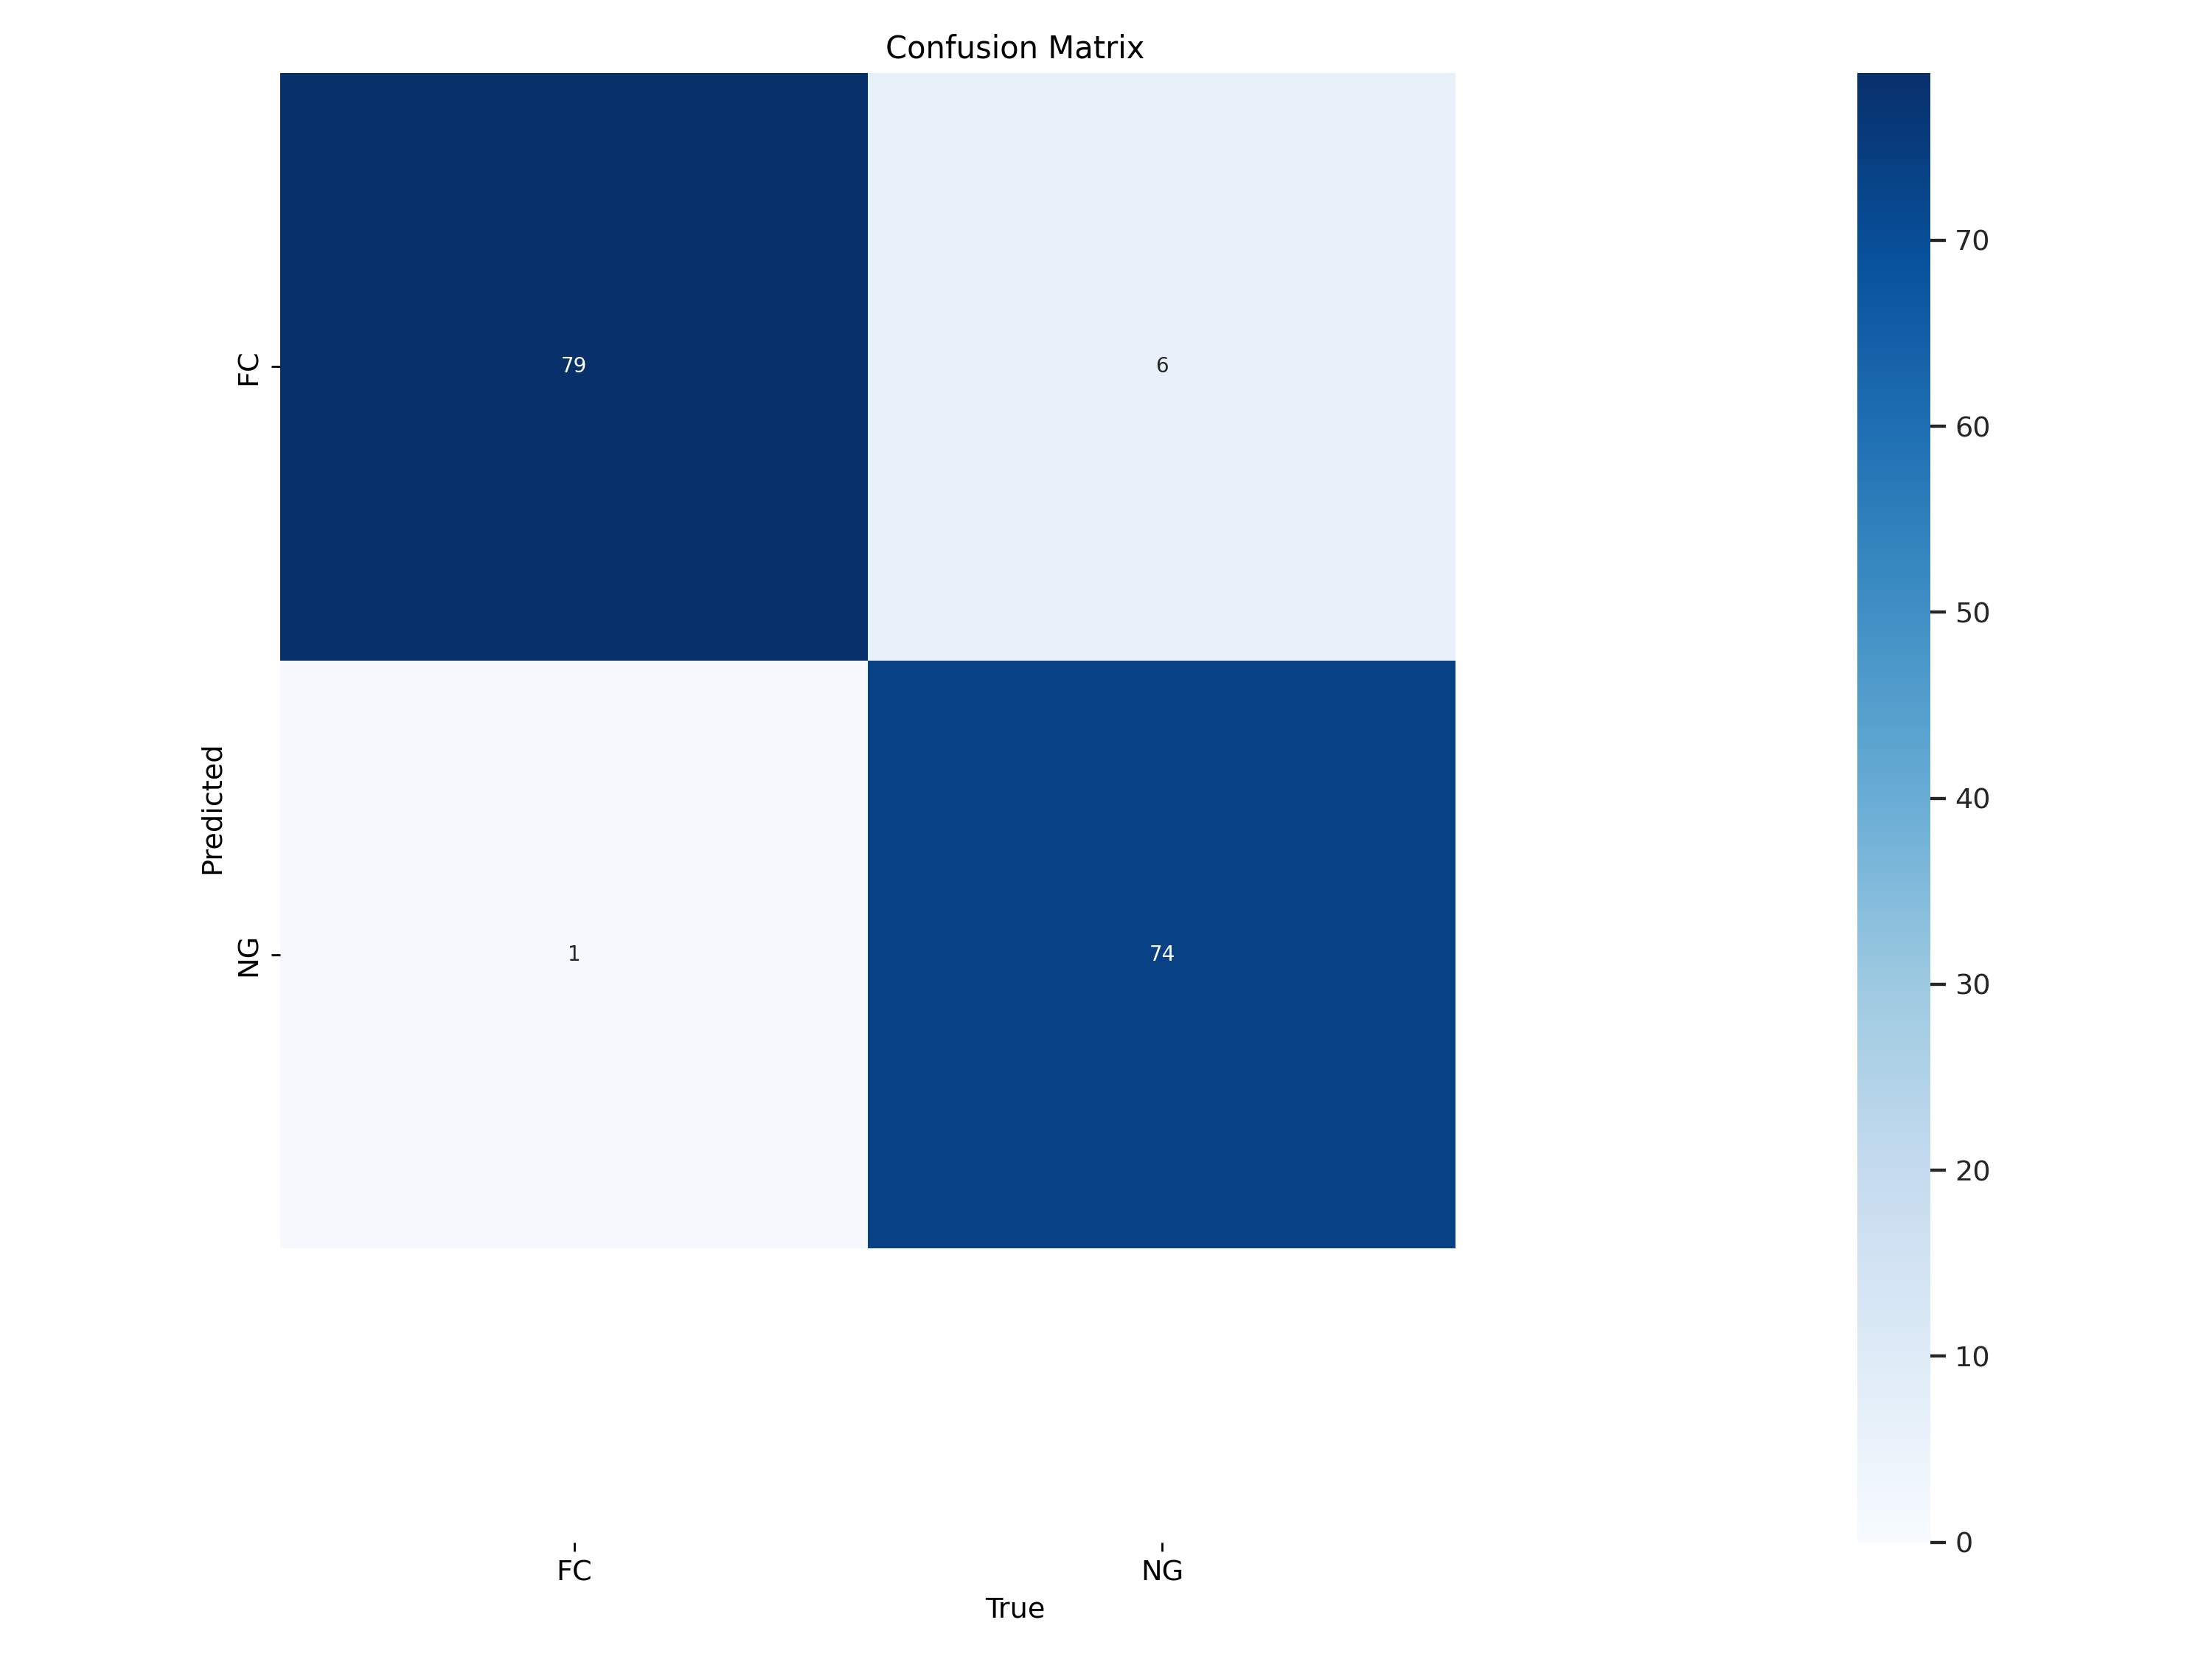
\includegraphics[width=1.3\linewidth]{Rohit_Master_Thesis//Images/yolov8m_confusion_matrix.png}
    \caption{Confusion matrix for the baseline model \gls{yolo}v8-M, its accuracy is 93.75\%}
    \label{fig:yolov8m confusion matrix}
\end{figure}

The confusion matrix in figure \ref{fig:yolov8m confusion matrix} shows almost similar results to that of \gls{yolo}v8-L. With 79 True positives and 74 true negatives, while only making 6 false positives and 1 false negative predictions, apart from the 1 misclassified normal image as anomalous the results are similar to that of \gls{yolo}v8-L. This indicates that the \gls{yolo}v8-M performance though highly accurate, but still falls just short of \gls{yolo}v8-L's performance due to its smaller capacity for learning complex patterns. As can be seen from the table \ref{tab:yolov8_performance}, the model achieved a precision of 0.9867, meaning that almost all of the predictions of normal(FC) images were correct. The recall for both the \gls{yolo}v8-L and \gls{yolo}v8-M matches and is equal to 0.925, indicating that both the models were able to successfully detect same number of FC cases. The F1-score of the model was 0.9547, which is slightly lower than \gls{yolo}v8-L, due to the small decrease in the precision. While the model was highly accurate, it did produce a small number of false positives, in this case 6 anomalous(NG) images were misclassified as normal(FC), which reduced it's precision slightly.

%See if you need to include loss and accuracy curve for both the models of YOLO

%Probably for discussion section(remember to paraphrase)
%Explanation of Results

%YOLOv8-M strikes a balance between computational efficiency and accuracy. The model achieves 93.75\% accuracy, which is competitive given its smaller architecture compared to YOLOv8-L. The slightly lower performance is expected due to YOLOv8-M’s reduced depth and number of parameters, which limits its ability to capture as many intricate patterns in the data as YOLOv8-L. However, YOLOv8-M’s simpler structure makes it faster and more computationally efficient, making it suitable for tasks where real-time performance and resource limitations are important.

%Model Comparison and Insights
%YOLOv8-L outperforms YOLOv8-M by achieving 95\% accuracy, compared to YOLOv8-M’s 93.75\%. This difference in performance can be attributed to the larger number of layers and parameters in YOLOv8-L, which allows it to capture more detailed features from the dataset. YOLOv8-L’s larger architecture is particularly beneficial for classification tasks that involve complex patterns or subtle differences between classes, making it a better choice for applications where accuracy is critical.

%However, YOLOv8-M offers significant advantages in terms of speed and computational efficiency. Despite having fewer layers, YOLOv8-M achieves strong results, making it a good option for scenarios where real-time inference is necessary or where computational resources are limited. The slight trade-off in accuracy is reasonable given the gains in efficiency, making YOLOv8-M ideal for environments where fast processing is prioritized over achieving the highest possible accuracy.

\paragraph*{\gls{dfm} : }

In this section, we will look into the results obtained from various experiments using \gls{dfm}. \gls{dfm} is explained in the section \ref{subsec:dfm}, and in our experiments, we evaluated \gls{dfm} performance using various backbones, their layers, and pooling techniques to explore the robustness and accuracy of the model. Below the results are divided based on the backbone used. 

\textbf{ResNet50} : Here we used ResNet50's layer4 for feature extraction along with \gls{nll} as the scoring type. This gave us the \gls{auroc} score of 0.6309 and F1-score of 0.6689, with an overall accuracy of 50.7\% which is not very good as can be seen from the table \ref{tab:dfm resnet results}, its basically doing random guessing. The low F1-score suggests that while the model was good at detecting anomalies, it struggled with precision due to the high number of false positives. These findings suggests that using features extracted from higher layers like layer4, may have led the model to focus on more abstract, high-level features which are less effective at determining anomalies from normal samples.

\begin{table}[ht!]
    \centering
    \begin{tabular}{|l|c|c|c|c|c|}
        \hline
        \textbf{Model} & \textbf{Accuracy (\%)} & \textbf{\gls{auroc}} &\textbf{Precision} & \textbf{Recall} & \textbf{F1-score} \\ \hline
        ResNet50 & 50.71\% & 0.6309 & 0.5036 & 1.0 & 0.6699 \\ \hline
        Wide-ResNet50-2 (layer2, nll) & 60\% & 0.6382 & 0.5556 & 1.0 & 0.7143 \\ \hline
        Wide-ResNet50-2 (layer2, fre) & 62.12\% & 0.5795 & 0.5681 & 1.0 & 0.7254 \\ \hline
        Wide-ResNet50-2 (layer3) & 62.86\% & 0.7265 & 0.5738 & 1.0 & 0.7292 \\ \hline
    \end{tabular}
    \caption{Results for ResNet and Wide-ResNet50-2 Backbones}
    \label{tab:dfm resnet results}
\end{table}

Another configuration which we tried was using a different variant of ResNet50 called Wide-ResNet50-2 and performing feature extraction using the layer2, while keeping the \gls{pca} level at 0.97 and using \gls{nll} score type. This configuration resulted in slight improvement in both the accuracy and \gls{auroc} score of 60\% and 0.6382 respectively. The precision improved to 0.5556, while the recall stayed at 1.0, resulting in an F1-score of 0.7143 as shown in the table \ref{tab:dfm resnet results}. Along with that, we also performed similar experiment by keeping the backbone and layer same, but changing the \gls{pca} level to 0.995 and scoring type to \gls{fre}. This resulted in much better compared to when we used scoring type as \gls{nll}, where accuracy increased by about 2\% to 62.12\% while seeing a drop in \gls{auroc} to 0.5795. The recall stayed the same at 1.0, but a slight increase in precision was observed to 0.5681, therefore increasing the F1-score to 0.7254. This improvement in both precision and F1-score shows that lower-level features from layer2 were more effective at capturing variations between normal and anomalous images. Finally, with seeing better result with \gls{fre} scoring type, we experimented with one more layer of the same backbone, the layer here used was layer3, with this we again saw slight improvement across all the metrics, the accuracy came out to be 62.86\% which is a small incremental update, while with \gls{auroc} score we saw an improvement of about 25\% when compared to Wide-ResNet50-2 (layer2, \gls{fre}) of the table \ref{tab:dfm resnet results}, and saw a rise of about 14\% when compared with Wide-ResNet50-2 (layer2, \gls{nll}).Other layers were also tried for both the ResNet50 and Wide-ResNet50-2 backbone, but all of them resulted in the model just random guessing the predictions i.e. the accuracy was 50\%.

\textbf{Densenet} : 

Next, we conducted experiments using different DenseNet backbones. Firstly, we used DenseNet121, which extracted features from the features.norm5 layer and the \gls{fre} score type. This configuration improved the models performance further, with an \gls{auroc} score of 0.7309 and an accuracy of 61.43\%. The model reached a precision of 0.5645 and a recall of 1.0, giving an F1-score of 0.7216. These improved scores suggests that the DenseNet architecture, which relies on dense connections and feature reuse, contributed to improved feature representations for anomaly detection. Table \ref{tab:dfm densenet results} shows the results of different backbones of DenseNet.

\begin{table}[ht!]
    \centering
    \begin{tabular}{|l|c|c|c|c|c|}
        \hline
        \textbf{Model} & \textbf{AUROC} & \textbf{Accuracy} & \textbf{Precision} & \textbf{Recall} & \textbf{F1-score} \\ \hline
        DenseNet121 & 0.7310 & 0.6143 & 0.5645 & 1.0 & 0.7216 \\ \hline
        DenseNet169 (norm5) & 0.7456 & 0.6571 & 0.5932 & 1.0 & 0.7447 \\ \hline
        \textbf{DenseNet169 (denseblock3, 0.97 PCA)} & \textbf{0.7203} & \textbf{0.7286} & 0.6538 & 0.9714 & 0.7816 \\ \hline
        DenseNet169 (denseblock3, 0.995 PCA) & 0.7190 & 0.7214 & 0.6422 & 1.0 & 0.7821 \\ \hline
        DenseNet201 (denseblock3, 0.995 PCA) & 0.7259 & 0.7143 & 0.6389 & 0.9857 & 0.7753 \\ \hline
        %DenseNet264d (untrained) & 0.8029 & N/A & N/A & N/A & 0.8471 \\ \hline
        %DenseNet201 (denseblock3, 0.97 PCA) & 0.7265 & N/A & N/A & N/A & 0.8460 \\ \hline
    \end{tabular}
    \caption{Results for DenseNet Backbones}
    \label{tab:dfm densenet results}
\end{table}

The best performing configuration for the DenseNet architecture, comes from the DenseNet169 backbone, with features extracted from features.denseblock3 layer, a \gls{pca} level of 0.97, and the \gls{fre} score type as shown in the table \ref{tab:dfm densenet results}. This configuration gave an \gls{auroc} score of 0.7203 and an accuracy of 72.86\%. Precision also improved to 0.6538, while recall reduced slightly still remaining high at 0.9714, resulting in a F1-score of 0.7816. This improvement in both precision and F1-score suggests that the DenseNet169's larger size allowed for better feature extraction and classification, particularly when extracting features from the third dense block. The high recall score indicates that the model was able to detect most of the anomalies as can be seen in the confusion matrix \ref{fig:dfm densenet169 confusion matrix}, while the increase in precision value indicates a significant decrease in the number of false positives when compared to other configurations.

\begin{figure}[ht!]
    \centering
    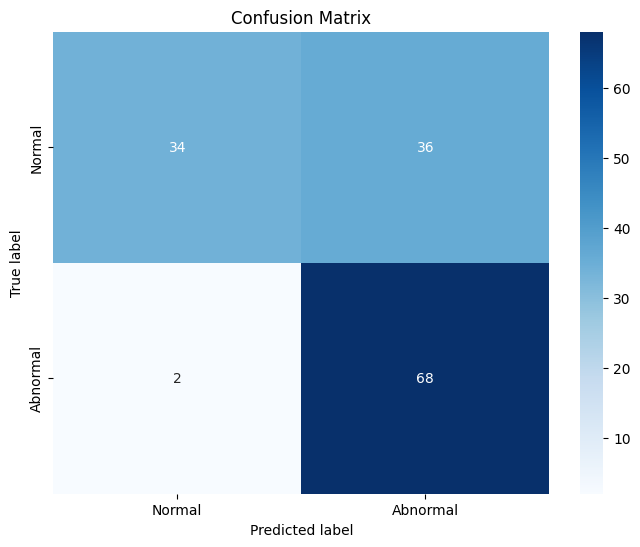
\includegraphics[width=1\linewidth]{Rohit_Master_Thesis//Images/dfm_densenet_best_confusion_matrix.png}
    \caption{Confusion matrix for the best performing configuration for \gls{dfm} model with DenseNet169 backbone, its accuracy is 72.86\%}
    \label{fig:dfm densenet169 confusion matrix}
\end{figure}

After getting good results with the configuration explained above, we thought of checking another variation of the DenseNet169 backbone, with keeping the feature extraction layer and scoring type same as before, but using a higher \gls{pca} level of 0.995, allowing for greater variance in the data. But the results were more or less similar to the previous configuration, with a slightly lower \gls{auroc} of 0.7190 and an accuracy of 72.14\%, along with precision of 0.6422 and an F1-score of 0.7821. The recall remained at 1.0, but the decrease in precision compared to the previous configuration indicates that the increase in retained variance caused the model to classify a higher number of normal images as anomalous. Finally, DenseNet201 was also tested with same feature extraction layer and keeping the other hyperparameters same as well. This configuration also gave very similar results to previous ones which are highlighted in the table \ref{tab:dfm densenet results}.


% In discussions explain also the difference between scoring type fre and nll
% In discussion also discuss why was the recall for most part 1.0

\paragraph*{\gls{dfkde} : }

Here we discuss the results obtained for the model \gls{dfkde}. It combines the power of \gls{dl} with statistical methods like \gls{pca} and \gls{kde}. The model first extracts robust features using a pretrained deep neural network, then reducing their dimensionality by using \gls{pca}, and finally applying \gls{kde} to model the distribution of normal data. Two backbones were tested in this experiments namely ResNet18 and Wide-ResNet50. The overview of the results for different configurations in the form of bar chart is shown in the figure \ref{fig:dfkde model results}.

\begin{figure}[ht!]
    \centering
    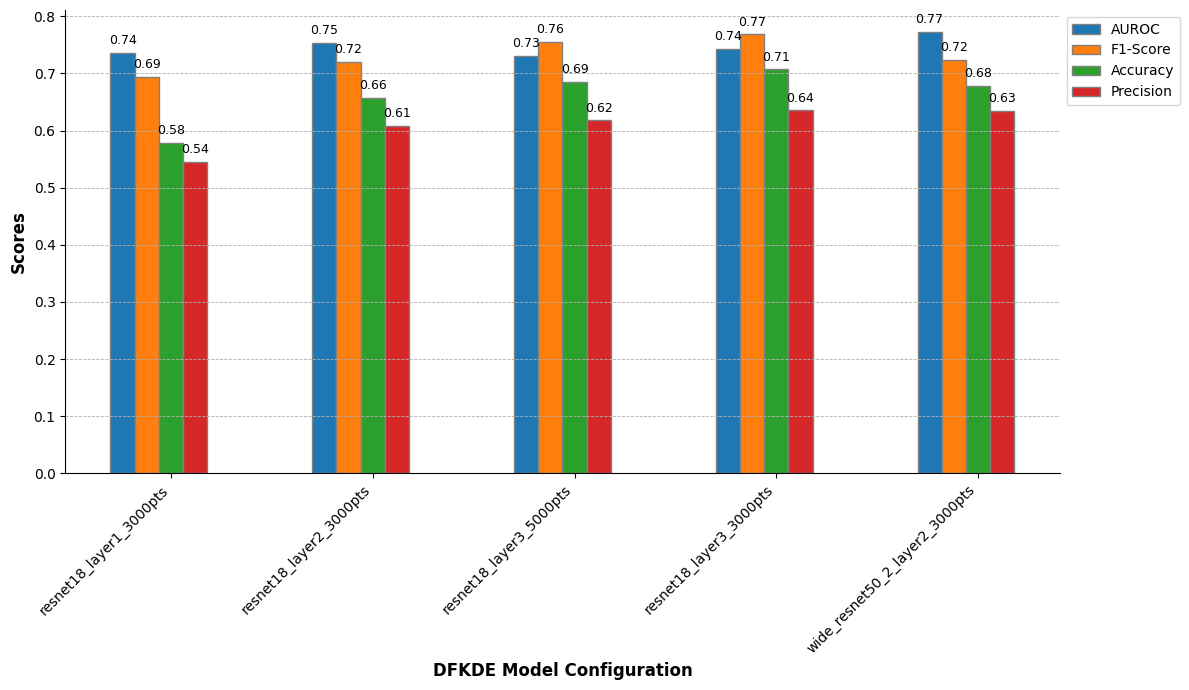
\includegraphics[width=1.2\linewidth]{Rohit_Master_Thesis//Images/dfkde_model_results.png}
    \caption{DFKDE model results for different backbones. The values shown here include \gls{auroc} score, F1-score, accuracy, and precision.}
    \label{fig:dfkde model results}
\end{figure}

\textbf{ResNet18} : 

For the first experiment with ResNet18 backbone, we use the feature extraction layer1. This configuration aims at capturing the lower level basic features, and its trained with a maximum of 3000 training points to fit the \gls{kde} model.

Its results are showed in the table \ref{tab:dfkde resnet18 results}. As can be seen, the performance is not quite good, with \gls{auroc} score of 0.7364 and an accuracy of 57.86\%. Precision is quite low at 0.5447, while recall is high at 0.9571, resulting in an F1-score of 0.6943. The lower precision value indicates that the features extracted from lower layer leads to introduction of noise, leading to higher false positives. While the high recall value suggests that the model was still able to detect most of the anomalies correctly. But still the overall performance of the model suffered as low-level features are less effective in anomaly detection for \gls{dfkde} model.

\begin{table}[ht!]
    \centering
    \begin{tabular}{|l|c|c|c|c|c|c|}
        \hline
        \textbf{Layer} & \textbf{AUROC} & \textbf{Accuracy(\%)} & \textbf{Precision} & \textbf{Recall} & \textbf{F1 Score} \\ \hline
        Layer1, max training points 3000 & 0.7364 & 57.86\% & 0.5447 & 0.9571 & 0.6943 \\ \hline
        Layer2, max training points 3000 & 0.7535 & 65.71\% & 0.6078 & 0.8857 & 0.7209 \\ \hline
        Layer3, max training points 3000 & 0.7428 & 70.71\% & 0.6355 & 0.9714 & 0.7684 \\ \hline
        Layer3, max training points 5000 & 0.7310 & 68.57\% & 0.6182 & 0.9714 & 0.7556 \\ \hline
    \end{tabular}
    \caption{Results for DFKDE Model with ResNet18 Backbone}
    \label{tab:dfkde resnet18 results}
\end{table}

For the second experiment with ResNet18 backbone, we used feature extraction layer2, the number of maximum data points for \gls{kde} model remained the same as like before at 3000.

The model achieved an \gls{auroc} score of 0.7535 which is slightly better than when features were extracted from layer1, an accuracy of 65,71\% is observed, which is about 14\% higher than that of configuration 1, as can be seen in the table \ref{tab:dfkde resnet18 results}. A precision of 0.6078, and a recall of 0.8857, resulting in an F1-score of 0.7209. This improvement in \gls{auroc} score and precision indicates that the mid-level features are more effective in anomaly detection for \gls{dfkde} model as they maintain balance of the low-level details and high-level semantic information. Even though recall slightly reduced compared to layer1, but the improvement in precision indicates a reduction in false positives.

For the third experiment, we select layer3 for feature extraction of the backbone ResNet18, which is responsible for capturing higher-level semantic information. This layer offers a more abstract representation of the input data, which can be particularly suitable for anomaly detection tasks. This configuration was the best performing one in the \gls{dfkde} model.

As shown in the table \ref{tab:dfkde resnet18 results} an \gls{auroc} score of 0.7427, an accuracy of 70.71\% which is more than 22\% higher than configuration 1, and more than 7\% higher than configuration 2. A further improvement in precision was observed at 0.6355, and a recall of 0.9714, leading to an F1-score of 0.7684. The layer3 features gives more abstract representations of the data, which helped reduce false positive rate further while also maintaining high recall. However, a slight dip in \gls{auroc} compared to layer2 configuration can indicate that while the high-level features are useful, they might lack some of the finer details necessary for achieving good anomaly detection performance.

%\subsection{Layer wise performance comparison}

%\subsection{Performance on NG images}

%\subsection{Performance on FC images}

\subsection{Discussion}

% In discussions explain also the difference between scoring type fre and nll
% In discussion also discuss why was the recall for most part 1.0

%Probably for discussion section(remember to paraphrase)
%Explanation of Results

%YOLOv8-M strikes a balance between computational efficiency and accuracy. The model achieves 93.75\% accuracy, which is competitive given its smaller architecture compared to YOLOv8-L. The slightly lower performance is expected due to YOLOv8-M’s reduced depth and number of parameters, which limits its ability to capture as many intricate patterns in the data as YOLOv8-L. However, YOLOv8-M’s simpler structure makes it faster and more computationally efficient, making it suitable for tasks where real-time performance and resource limitations are important.

%Model Comparison and Insights
%YOLOv8-L outperforms YOLOv8-M by achieving 95\% accuracy, compared to YOLOv8-M’s 93.75\%. This difference in performance can be attributed to the larger number of layers and parameters in YOLOv8-L, which allows it to capture more detailed features from the dataset. YOLOv8-L’s larger architecture is particularly beneficial for classification tasks that involve complex patterns or subtle differences between classes, making it a better choice for applications where accuracy is critical.

%However, YOLOv8-M offers significant advantages in terms of speed and computational efficiency. Despite having fewer layers, YOLOv8-M achieves strong results, making it a good option for scenarios where real-time inference is necessary or where computational resources are limited. The slight trade-off in accuracy is reasonable given the gains in efficiency, making YOLOv8-M ideal for environments where fast processing is prioritized over achieving the highest possible accuracy.

%Probably for discussion section(remember to paraphrase)
%Explanation of Results
%The performance of YOLOv8-L is in line with its design as a larger, more powerful model. The depth and complexity of the YOLOv8-L architecture allow it to capture a wide variety of patterns and features in the data, leading to its high precision and recall. The non-maximum suppression (NMS) technique used in YOLOv8 helps further refine the predictions by ensuring that overlapping bounding boxes are filtered, resulting in more accurate object classification. Additionally, YOLOv8-L's anchor-free detection mechanism improves its ability to generalize across objects of various sizes, contributing to its robustness in detecting NG and FC items.


% In DFM resnet results why changing the PCA_level and scoring type to fre resulted in better results?

%Discussion of Results and Insights for DFM

%The results of the experiments provide valuable insights into how the choice of backbone network, feature extraction layer, and scoring method influence the performance of the DFM model. Across all configurations, the model demonstrated high recall values, indicating its strong ability to detect anomalous samples. However, the key challenge in most configurations was improving precision, as many configurations suffered from high false-positive rates. This imbalance between precision and recall was most noticeable in configurations that used higher-level feature layers, such as layer4 in ResNet50, which may have caused the model to focus on abstract features less relevant for anomaly detection.

%The use of PCA for dimensionality reduction also played a crucial role in balancing the model’s performance. A PCA level of 0.97 generally provided a good balance between computational efficiency and information retention, while increasing the PCA level to 0.995 resulted in slightly higher overfitting and a decrease in precision. Additionally, the frequentist score type consistently outperformed the negative log-likelihood score in anomaly detection tasks, as it provided a more robust measure of the distance between the new data points and the normal data distribution.

%In conclusion, the DFM model’s performance varied significantly across different configurations. The best-performing setup used DenseNet169 with features extracted from DenseBlock3, a PCA level of 0.97, and the frequentist score type, achieving a balance between high precision and recall while maintaining a high sensitivity to anomalies. Future work could explore the integration of attention mechanisms or ensemble methods to further improve precision and reduce the false-positive rate, particularly in configurations that show a tendency to misclassify normal samples as anomalies.

%I can add diagram showing the performance according to layers
